\chapter{Implementación}

\section{Stack tecnológico}

La implementación de Nuvlo se ha realizado con un stack JavaScript/Node orientado a desarrollo web moderno. En el cliente se usa React para construir la interfaz y Vite como herramienta de desarrollo y empaquetado~\cite{ReactDocs,ViteDocs}. En el servidor se usa Node.js con Express para exponer la API HTTP~\cite{NodeDocs,ExpressDocs}. La capa de datos se apoya en Prisma como ORM y PostgreSQL como base de datos relacional~\cite{PrismaDocs,PostgreSQLDocs}.

Redis se incorpora como servicio auxiliar para datos efímeros y operaciones de apoyo, mientras que Docker Compose facilita reproducir el entorno local con los servicios necesarios~\cite{RedisDocs,DockerComposeDocs}. Esta combinación permite mantener una separación clara entre la lógica de negocio, la interfaz y la infraestructura de desarrollo.

\section{Frontend}

El \textit{frontend} organiza la experiencia alrededor de varias vistas principales: entrada con Jira, \textit{dashboard}, tablero, alertas, actividad y configuración. El \textit{dashboard} muestra las métricas principales, gráficos y \textit{widgets} configurables. La navegación se ha ajustado para mantener coherencia con los prototipos de la memoria y para funcionar tanto en escritorio como en móvil.

Se han añadido transiciones visuales ligeras para que los cambios de vista, paneles y acciones clicables no produzcan una sensación de parpadeo. Estas animaciones son sencillas y no introducen dependencias pesadas, por lo que no afectan de forma significativa al rendimiento de la aplicación.

\section{Backend e integración con Jira}

El \textit{backend} encapsula la comunicación con Jira Cloud. Cuando el usuario inicia sesión, la aplicación redirige a Atlassian y recibe el resultado del flujo OAuth. A partir de esa sesión, el servidor puede consultar los recursos autorizados de Jira y sincronizar la información necesaria para calcular las métricas.

La integración no calcula las métricas consultando Jira en cada carga del \textit{dashboard}. En su lugar, sincroniza los datos relevantes, los persiste en PostgreSQL y después la aplicación consulta su propia base de datos. Esto mejora la estabilidad de la interfaz, reduce dependencia de la red y facilita auditar qué datos se usaron para obtener cada resultado.

\section{Métricas implementadas}

El sistema calcula \textit{WIP}, \textit{Velocity}, \textit{Lead Time} y \textit{Cycle Time}. \textit{WIP} representa el trabajo en curso según el estado de las incidencias visibles. \textit{Velocity} resume el trabajo completado por periodo o \textit{sprint}. \textit{Lead Time} y \textit{Cycle Time} se calculan a partir de fechas de creación, resolución y transiciones cuando la información está disponible.

En Jira real, la calidad de estas métricas depende de cómo se haya usado el tablero y de si existen transiciones suficientes en el historial. Por este motivo, el proyecto incluye también una demo \textit{offline} con datos controlados, útil para validar escenarios que en una instancia real recién creada pueden no tener todavía histórico suficiente.

\section{Alertas, actividad y retención de datos}

La fase de interfaz incluye reglas de alerta basadas en umbrales, notificaciones visuales y un registro de actividad. Las alertas permiten avisar al usuario cuando una métrica supera una condición definida. El registro de actividad guarda eventos de uso relevantes, como sincronizaciones, cambios de sesión, creación de reglas, activación de alertas y tareas de limpieza.

La política de retención diferencia entre datos persistentes, datos operativos y datos efímeros. PostgreSQL conserva la información necesaria para análisis e histórico: proyectos importados, incidencias, transiciones, métricas calculadas, reglas de alerta y sincronizaciones. Estos datos son los que permiten reconstruir el estado mostrado en el \textit{dashboard} y justificar los resultados obtenidos.

Redis se reserva para información temporal: estados del flujo OAuth, valores CSRF, verificadores PKCE, cachés de corta duración y datos auxiliares que no deben mantenerse indefinidamente. Estos elementos se almacenan con tiempo de vida limitado mediante TTL, de forma que expiran automáticamente sin requerir limpieza manual~\cite{RedisDocs}.

Para evitar crecimiento indefinido de la base de datos, los \textit{logs} de actividad y el historial de alertas se tratan como datos retenibles. La aplicación contempla tareas de limpieza que eliminan o archivan registros antiguos según una ventana configurable. De este modo, se mantiene la trazabilidad necesaria para depuración y auditoría básica sin convertir PostgreSQL en un almacén ilimitado de eventos.

\section{Diagrama de despliegue}

El diagrama de despliegue representa la distribución física prevista del sistema sobre nodos de ejecución. Según la notación UML, un nodo modela un recurso computacional o entorno de ejecución, un artefacto representa una unidad desplegable del sistema y las rutas de comunicación indican cómo se conectan dichos nodos durante la ejecución~\cite{OMGUML251}. En este trabajo se utiliza para mostrar cómo se ubican el cliente web, el \textit{backend}, la base de datos, la caché y los servicios externos de Atlassian.

\begin{figure}[htbp]
    \centering
    \makebox[\textwidth][c]{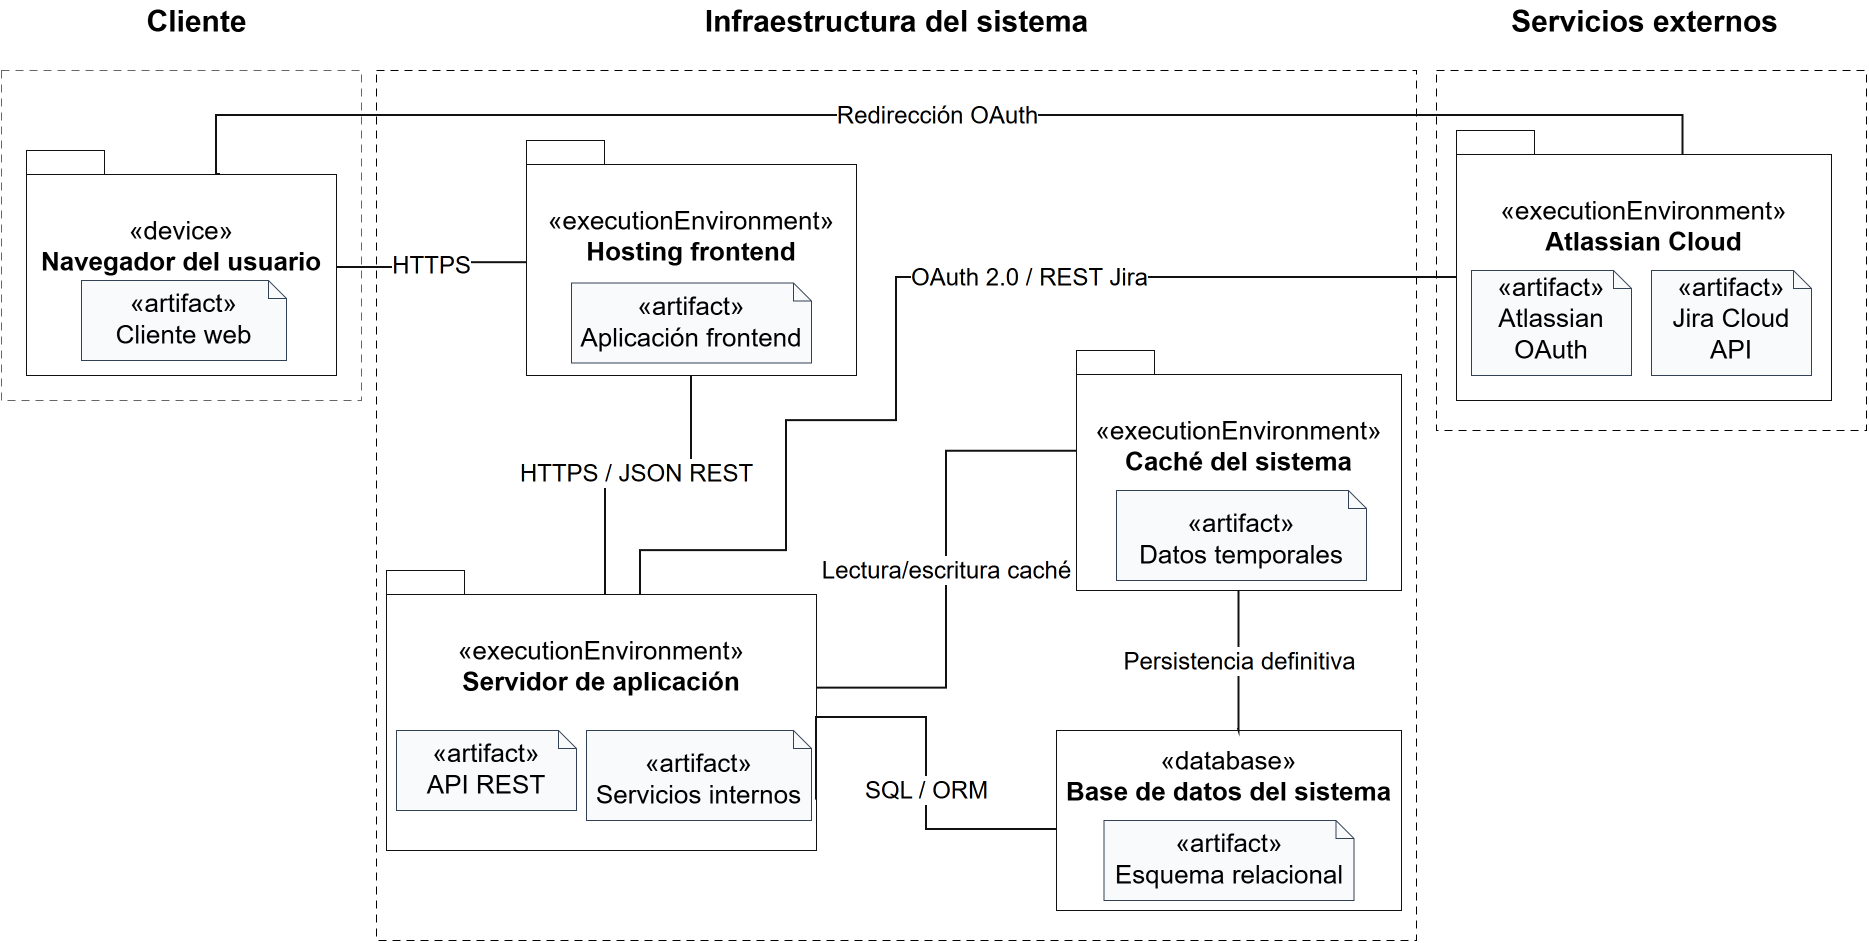
\includegraphics[width=1.25\textwidth]{diagrams/despliegue-sistema.png}}
    \caption{Diagrama de despliegue del sistema}
    \label{fig:despliegue-sistema}
\end{figure}

La Figura~\ref{fig:despliegue-sistema} distingue entre el cliente del usuario, la infraestructura propia del sistema y las dependencias externas. El usuario accede desde su navegador al \textit{frontend} mediante \texttt{HTTPS}; el \textit{frontend} consume la \texttt{API REST} del servidor de aplicación; y el \textit{backend} coordina la autenticación, sincronización, cálculo de métricas, gestión de alertas y acceso a datos.

\begin{itemize}
    \item \textbf{Navegador del usuario}: ejecuta el cliente web y muestra las vistas de panel, tablero, registro, alertas y configuración.
    \item \textbf{Servidor web / hosting \textit{frontend}}: aloja el artefacto \textit{frontend} compuesto por los recursos \texttt{HTML}, \texttt{CSS} y \texttt{JavaScript} de la aplicación.
    \item \textbf{Servidor de aplicación}: despliega la \texttt{API REST} y los servicios internos encargados de sesión, sincronización con Jira, cálculo de métricas y alertas.
    \item \textbf{Caché del sistema}: almacena temporalmente datos recientes de Jira, resultados de métricas o información de sesión para reducir lecturas repetidas y evitar recálculos innecesarios.
    \item \textbf{Base de datos del sistema}: conserva la información persistente, incluyendo datos sincronizados, configuraciones, métricas calculadas, alertas y \textit{logs}.
    \item \textbf{Atlassian Cloud}: agrupa los servicios externos usados por el sistema. \texttt{Atlassian OAuth} permite autenticar al usuario y \texttt{Jira Cloud API} proporciona los datos de proyectos, tableros, \textit{sprints} e incidencias.
\end{itemize}

Las rutas de comunicación muestran que el navegador puede ser redirigido a Atlassian durante la autenticación OAuth, mientras que el servidor de aplicación se comunica con Jira mediante peticiones \texttt{REST}. La caché se sitúa entre la lógica de aplicación y la persistencia para acelerar consultas frecuentes, pero la base de datos mantiene la información definitiva del sistema.
\clearpage
